\section{Evaluation} \label{evaluation} 
In this section we evaluate the performance of our system using various datasets. 
We report both the quality (error rate) and performance of our proposed method. 

\subsection{Setup}\label{subsec:setup}
We evaluate our deployment method in distributed environment consists of 11 nodes (1 master, 10 slaves).
Each node is running on an Intel Xeon 2.40 GHz 16 core processor and has 28 GB of dedicated memory for running our prototype.

We implement a prototype of our deployment method on top of Apache Spark \cite{zaharia2010spark}.
It uses the SGD implementation available in the machine learning library of Apache Spark.
To demonstrate the deployment platform designed two machine learning pipelines.

\textbf{Criteo pipeline.} 
The Criteo pipeline consists of 5 operations: missing value imputer, column indexer, one hot encoder, vectorizer, standard scaler, and logistic regression model trainer. 
The Terabyte Criteo click log dataset is used for benchmarking algorithms for clickthrough rate (CTR) prediction \cite{criteo-log}.
It contains \hl{24} days of user click logs. 
The dataset  contains 13 numerical and 26 categorical features. 
After applying the indexer and one hot encoding number of features increased to \hl{1,000,000}.

\textbf{XXX pipeline.}
For all of the classification datasets, we report the prequential error when receiving a new training instances \cite{gama2009issues} .

\textit{Deployment scenario.} 
Pipelines are trained on an initial part of the data and then continuously trained using the remaining of the data.
We define 3 different deployment scenarios.
\begin{itemize}
\item A: Periodical retraining with no statistics collection
\item B: Periodical retraining with statistics collection
\item C: Proactive training with statistics collection
\end{itemize}

For Criteo pipeline, the pipeline is retrained on a daily basis.

\subsection{Dynamic Evaluation Set}\label{dynamic-evaluation-set}


\subsection{Learning Rate Adaptation Method}
However, all of the above methods are defined methods are tested for batch training of the models.
To assess how effective these methods are on hybrid training (scenario C), we experimented the methods on Criteo Dataset.

\begin{figure}[H]
\begin{subfigure}{0.5\columnwidth}
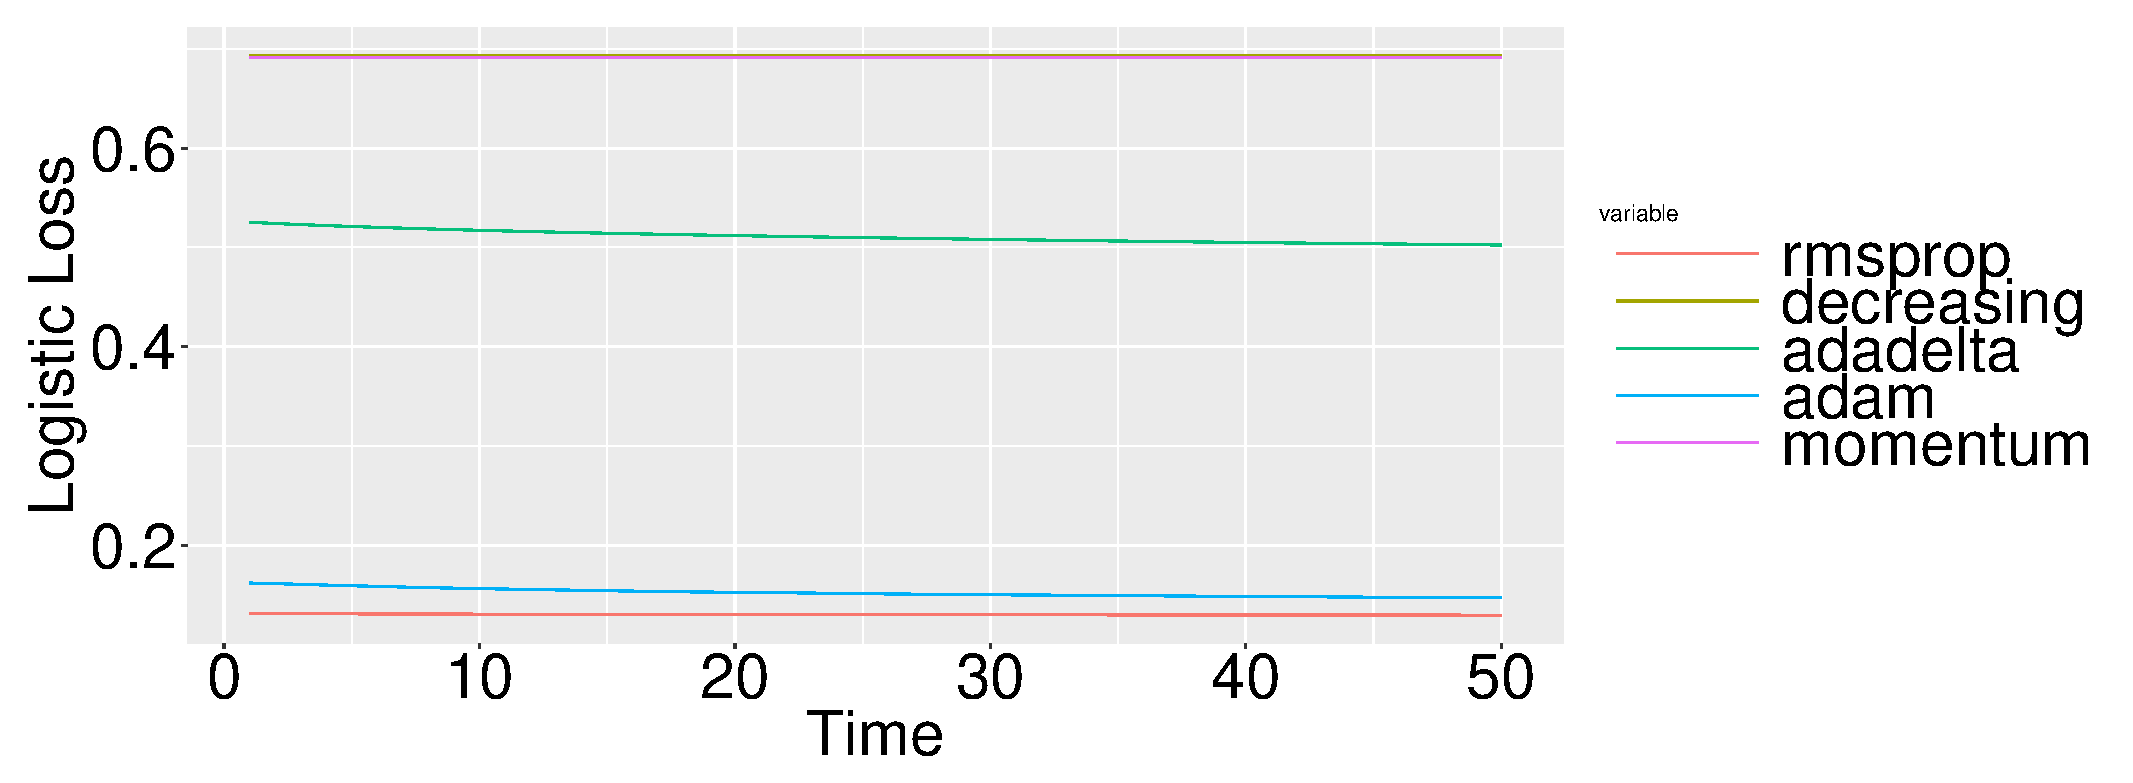
\includegraphics[width=\columnwidth]{../images/experiment-results/criteo-learning-rate-comparison-1.eps}
\caption{}
\label{fig:criteo-learning-rate-1}
\end{subfigure}%
\begin{subfigure}{0.5\columnwidth}
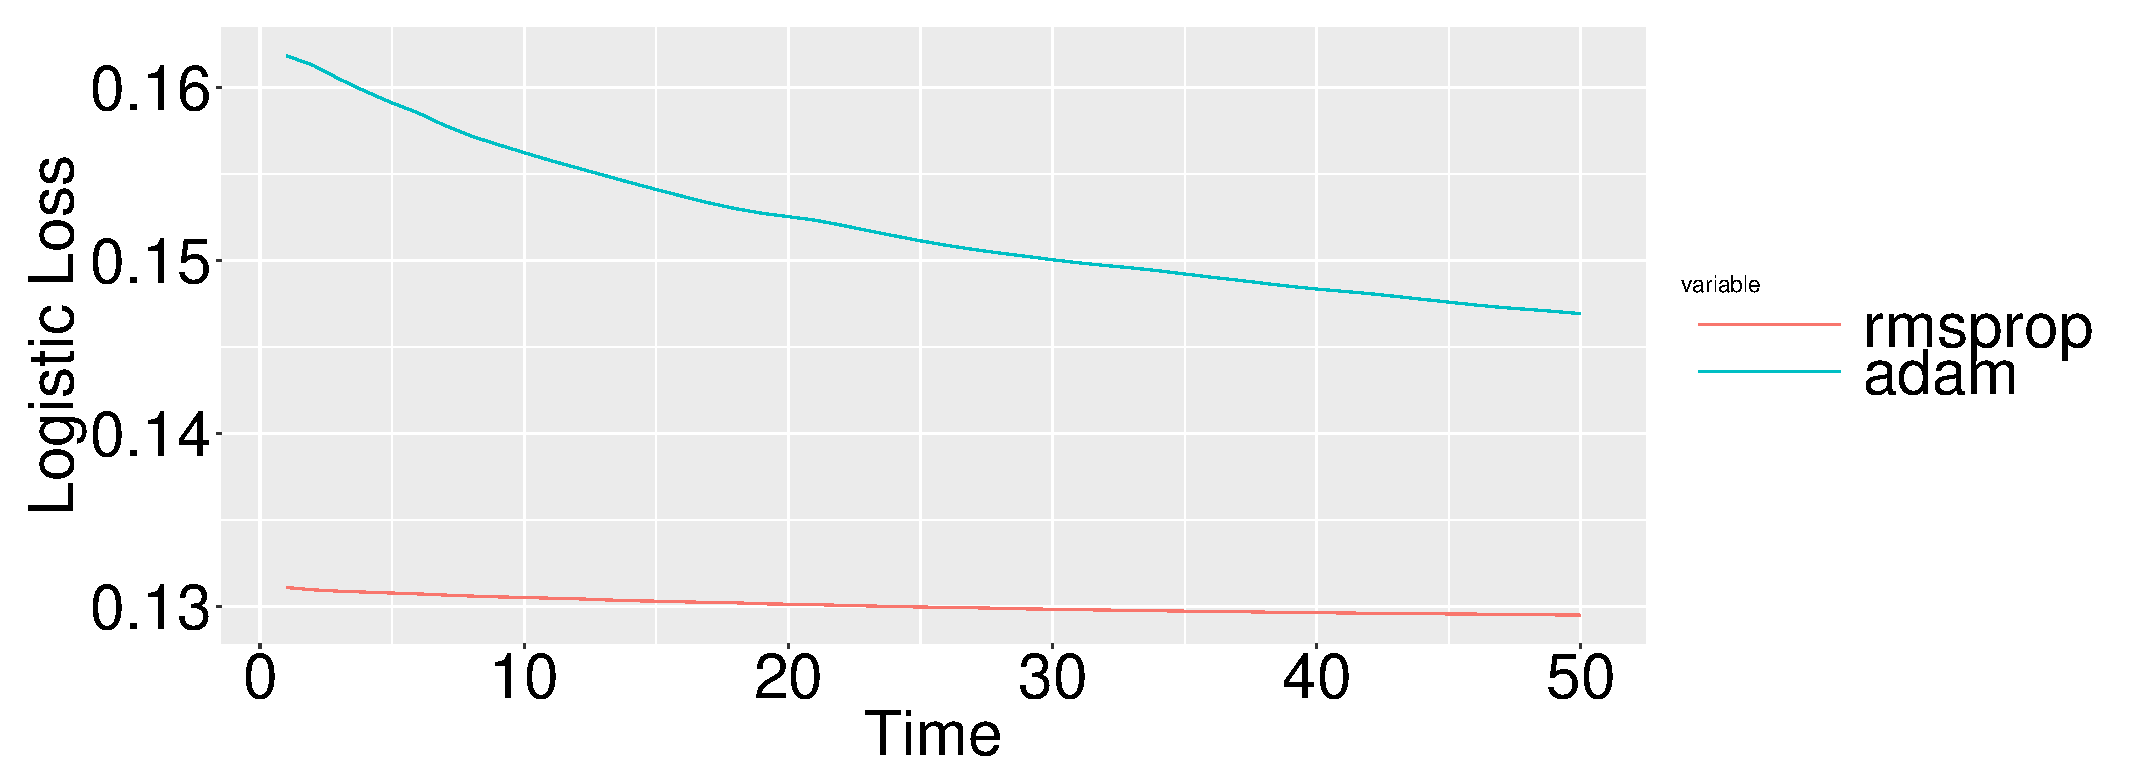
\includegraphics[width=\columnwidth]{../images/experiment-results/criteo-learning-rate-comparison.eps}
\caption{}
\label{fig:criteo-learning-rate}
\end{subfigure}
\vspace{2mm}
\caption{Different Learning rate adaptation methods for Continuous training of Criteo Pipeline}
\end{figure}

Figure \ref{fig:criteo-learning-rate-1} shows the log loss for different learning adaptation methods. 
\todo[inline]{All the methods except for rmsprop and adam seems not work properly without extensive grid search (or not working well at all). I should make sure there's no problem with the code and it is the algorithm that function poorly.}

\subsection{Sampling Methods}
\todo[inline]{redo this part, compare weighted time-based sampling vs random sampling different sizes}
In each iteration of SGD the data inside the buffer and a sample of the historical data is combined to update the model.
In this section, we investigate the effect of the sampling rate on the model quality and the running time of the system.
Figure \ref{fig:movie-lens-100k-sample-rate} shows that a larger sampling rate increases the quality of the model.
However, similar to the scheduling rate, the decrease in error rate is negligible considering the effect it has on running time. 
This is caused by the same phenomena, where the model after training on bigger sample rates start to converge faster.
As a result, bigger sample sizes do not have a considerable effect on the quality.
 
Figure \ref{fig:movie-lens-100k-sample-rate-time} shows the effect of increasing the sampling rate on the running time.
Increasing the sampling rate from 0.1 to 1.0, increases the running time by a factor of 5.
\todo[inline]{R3: . The sampling parameter deserves a more systematic treatment since it deeply affects the performance. In fact, Baseline+ and Velox represent two extreme settings of it: 0\% and 100\%. Instead, the paper simply suggests "setting the sampling rate to smaller values will increase the performance substantially, while only slightly affecting the quality of the model." It is not a sound conclusion if we agree Baseline+ is equivalent to 0\% sampling rate.}
Therefore, similar to the scheduling rate, setting the sampling rate to smaller values will increase the performance substantially, while only slightly affecting the quality of the model.

\textbf{Tuning parameters based on error rate:} The underlying machine learning model and the dataset have big effects on the selection of sampling rate and scheduling rate.
In the recommender system use case, due to the changes in the incoming data distribution, we see that bigger sample rates and higher scheduling rates have an effect (although small) on the quality of the model.
However, this is not be the case for every application.
To demonstrate this, we perform the same set of experiments on the MNIST dataset.
Figure \ref{fig:mnist-sample-rate} shows the effect of different sampling rates on the neural network classifier model for MNIST.
Contrary to the results we achieved for Movie Lens 100k, the error rates for different sampling rates are very similar.
This is caused by how neural networks behave.
Increasing the sampling rate causes similar data items to be used repeatedly in consecutive training iterations.
Neural networks are not affected by this oversampling, therefore the results are almost similar with different sampling rates.
Moreover, in this experiment, the number of parameters of the multi-layer perceptron is far less than the number of parameters of the matrix factorization model for Movie Lens 100k.
This causes the neural work to converge faster.
Therefore it is not affected by more training, unless new training observations arrive at the system.

\begin{figure}[h]
\begin{subfigure}{\columnwidth}
\centering
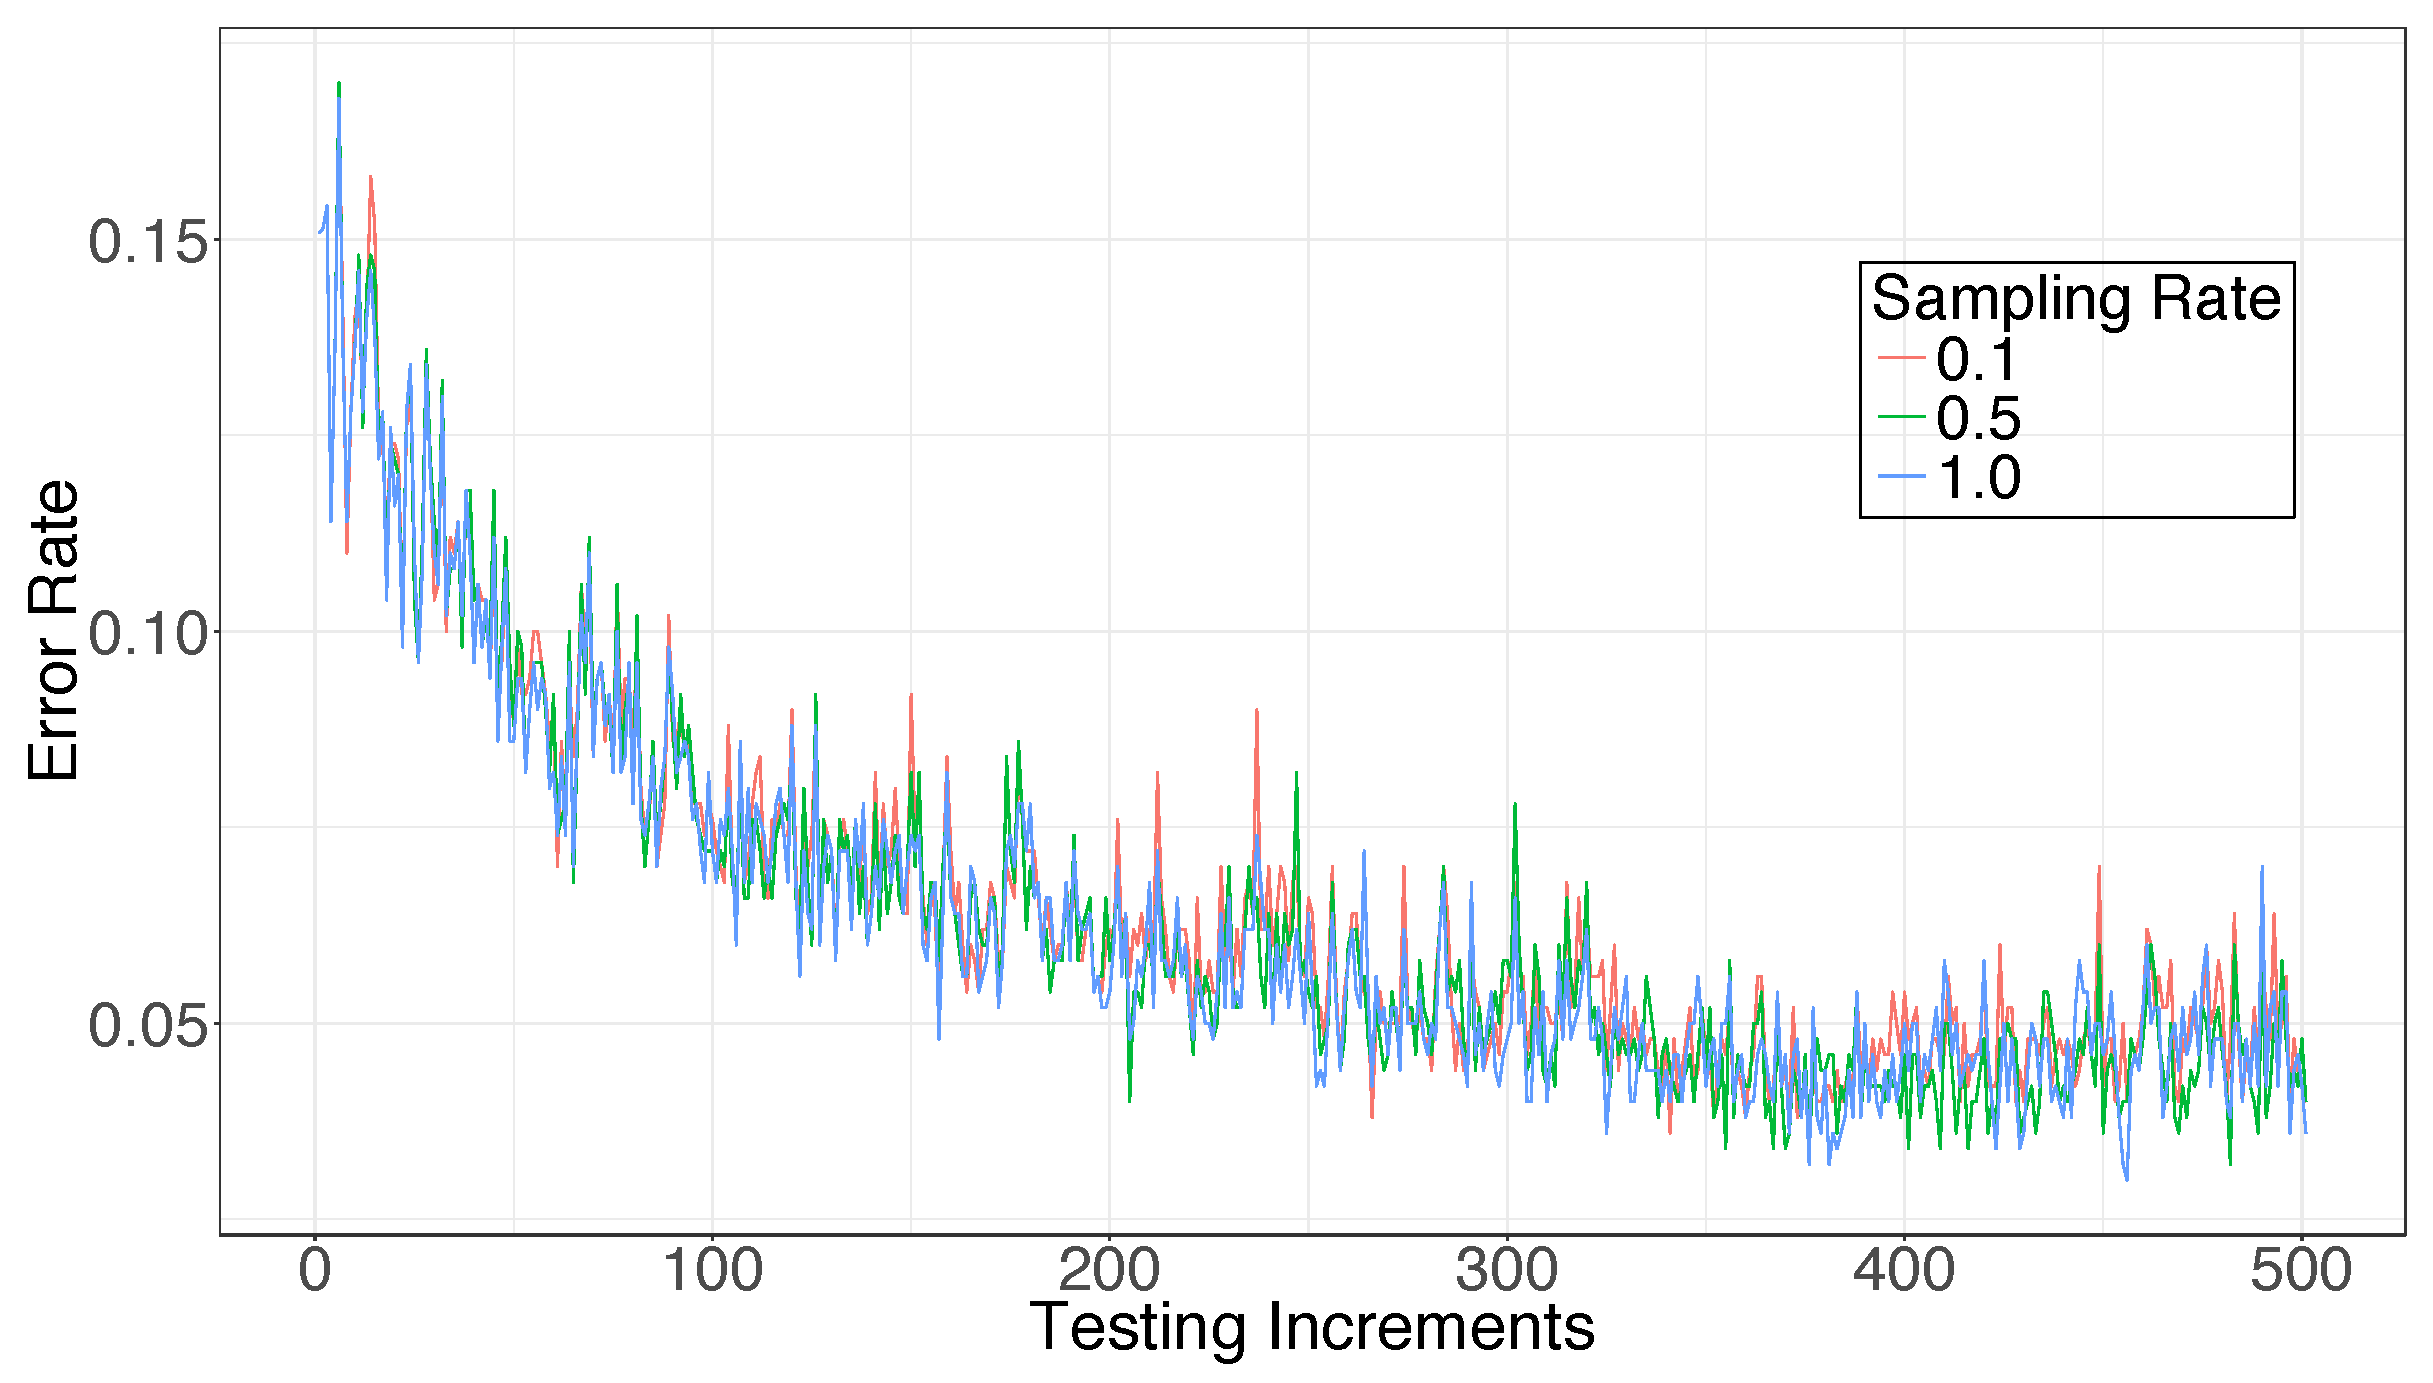
\includegraphics[width=\columnwidth]{../images/experiment-results/mnist-sampling-improved.eps}
\caption{Sampling rate}
\label{fig:mnist-sample-rate}
\end{subfigure}
\begin{subfigure}{\columnwidth}
\centering
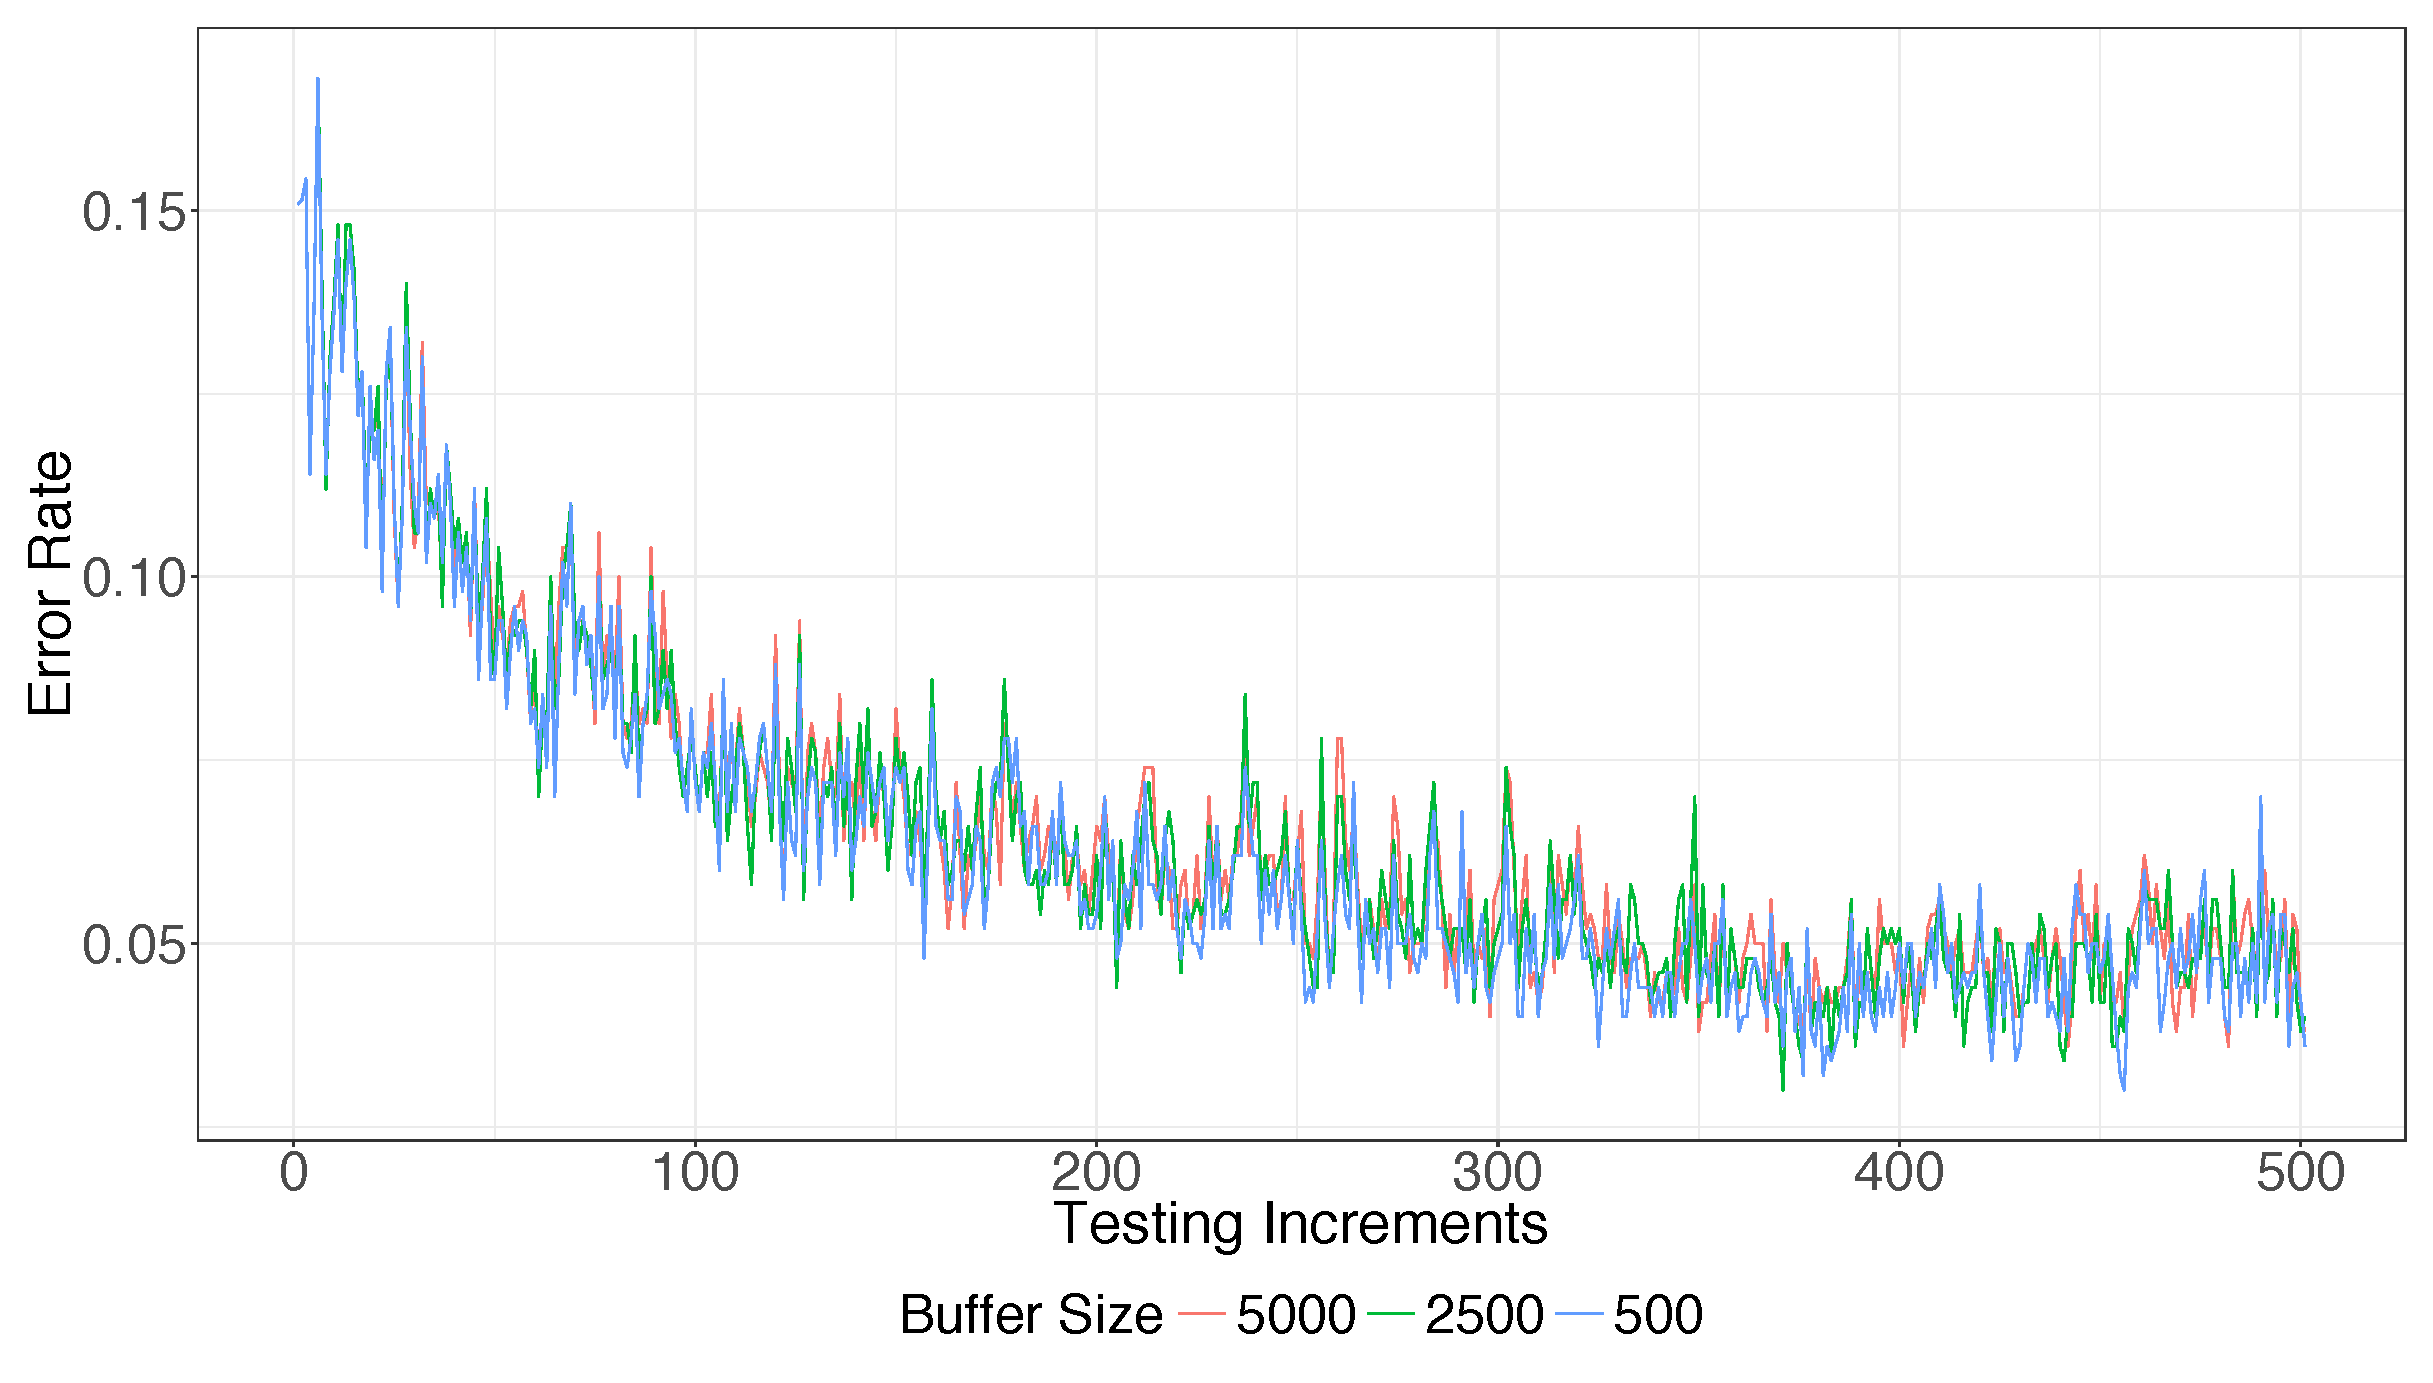
\includegraphics[width=\columnwidth]{../images/experiment-results/mnist-buffersize-improved.eps}
\caption{Buffer size}
\label{fig:mnist-buffer-size}
\end{subfigure}
\vspace{2mm}
\caption{Effect of Sampling and Scheduling Rate on Quality (MNIST)}
\end{figure}

Figure \ref{fig:mnist-buffer-size} shows how the buffer size affects the overall quality of the neural network model.
Similar to the sampling rate case, the error rate of the model is not affected by the scheduling rate.
New training observations that exist in the buffer have the maximum effect on the quality of the model since they are becoming available to the model for the first time.
As the scheduling rate increases, the number of new training observations remain the same, and only the historical data is used more frequently to train the model.
Since neural networks do not gain much benefit by revisiting the same items, increasing the scheduling rate has no effect on the overall quality.

Based on our findings, we conclude that increasing the sampling and scheduling rate does not always affect the quality.
In both the Movie Lens 100k and MNIST datasets, the change in scheduling and sampling rate have small to no effect on the overall quality.
However, the running time of the methods are heavily influenced by these parameters.
\todo[inline]{R3: Similarly, the treatment of buffer size is also shallow. "Setting these parameters to small values decreases the running time considerably and save computation resources regardless of the type of model the system is serving." What about setting the buffer size as 1? BD: Reviewer's confusion is because I have used both scheduling rate and buffer size in the text, although they both control how often a training iteration is executed, they are 'opposite' of each other. Increasing the scheduling rate means we have a smaller buffer size and decreasing the scheduling rate means we have a bigger buffer size. }
Setting these parameters to small values decreases the running time considerably and save computation resources regardless of the type of model the system is serving.

\subsection{Scheduling Policy}
\todo[inline]{redo this part using the criteo dataset}
This parameter specifies how often a new iteration of SGD should be scheduled. 
In our prototype, the scheduling rate is governed by a parameter called buffer size, which dictates how many new items should be stored in the buffer before a new iteration of SGD is executed. 
Executing one iteration of SGD, even using the entire data, is not a resource heavy process, and can be executed simultaneously with the serving component of the system. 

\begin{figure}[h]
\begin{subfigure}{\columnwidth}
\centering
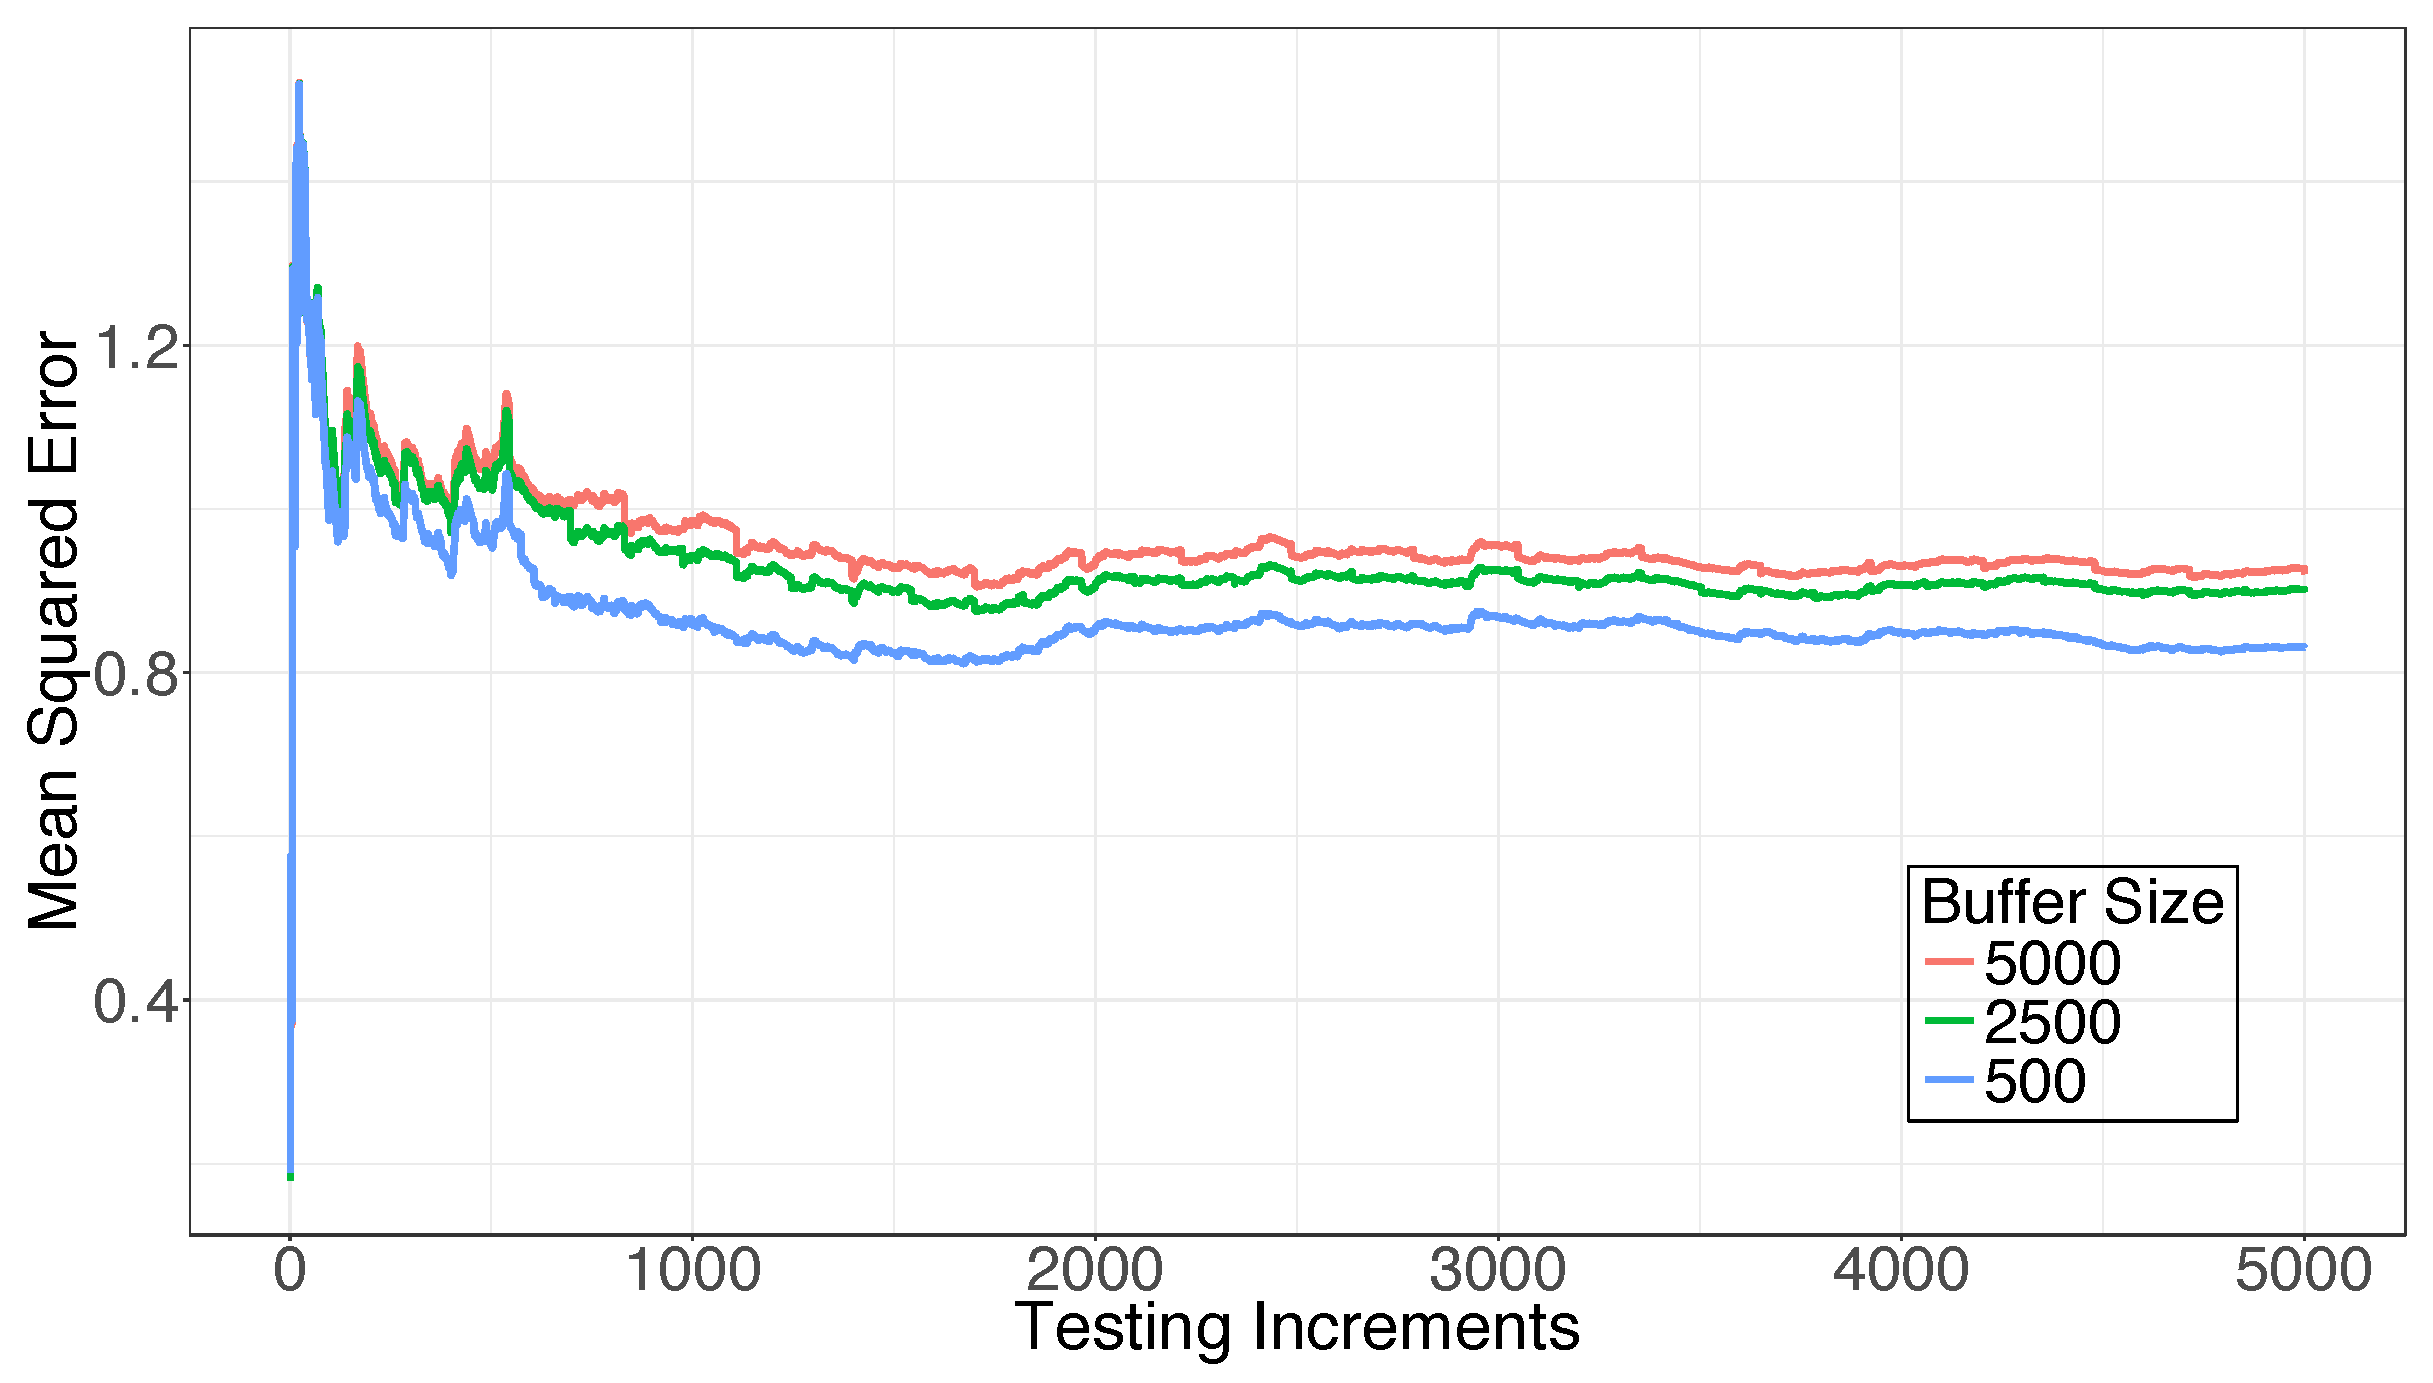
\includegraphics[width=\columnwidth]{../images/experiment-results/movie-lens-buffer-quality-improved.eps}
\caption{Buffer size}
\label{fig:movie-lens-100k-buffer-size-mse}
\end{subfigure}
\begin{subfigure}{\columnwidth}
\centering
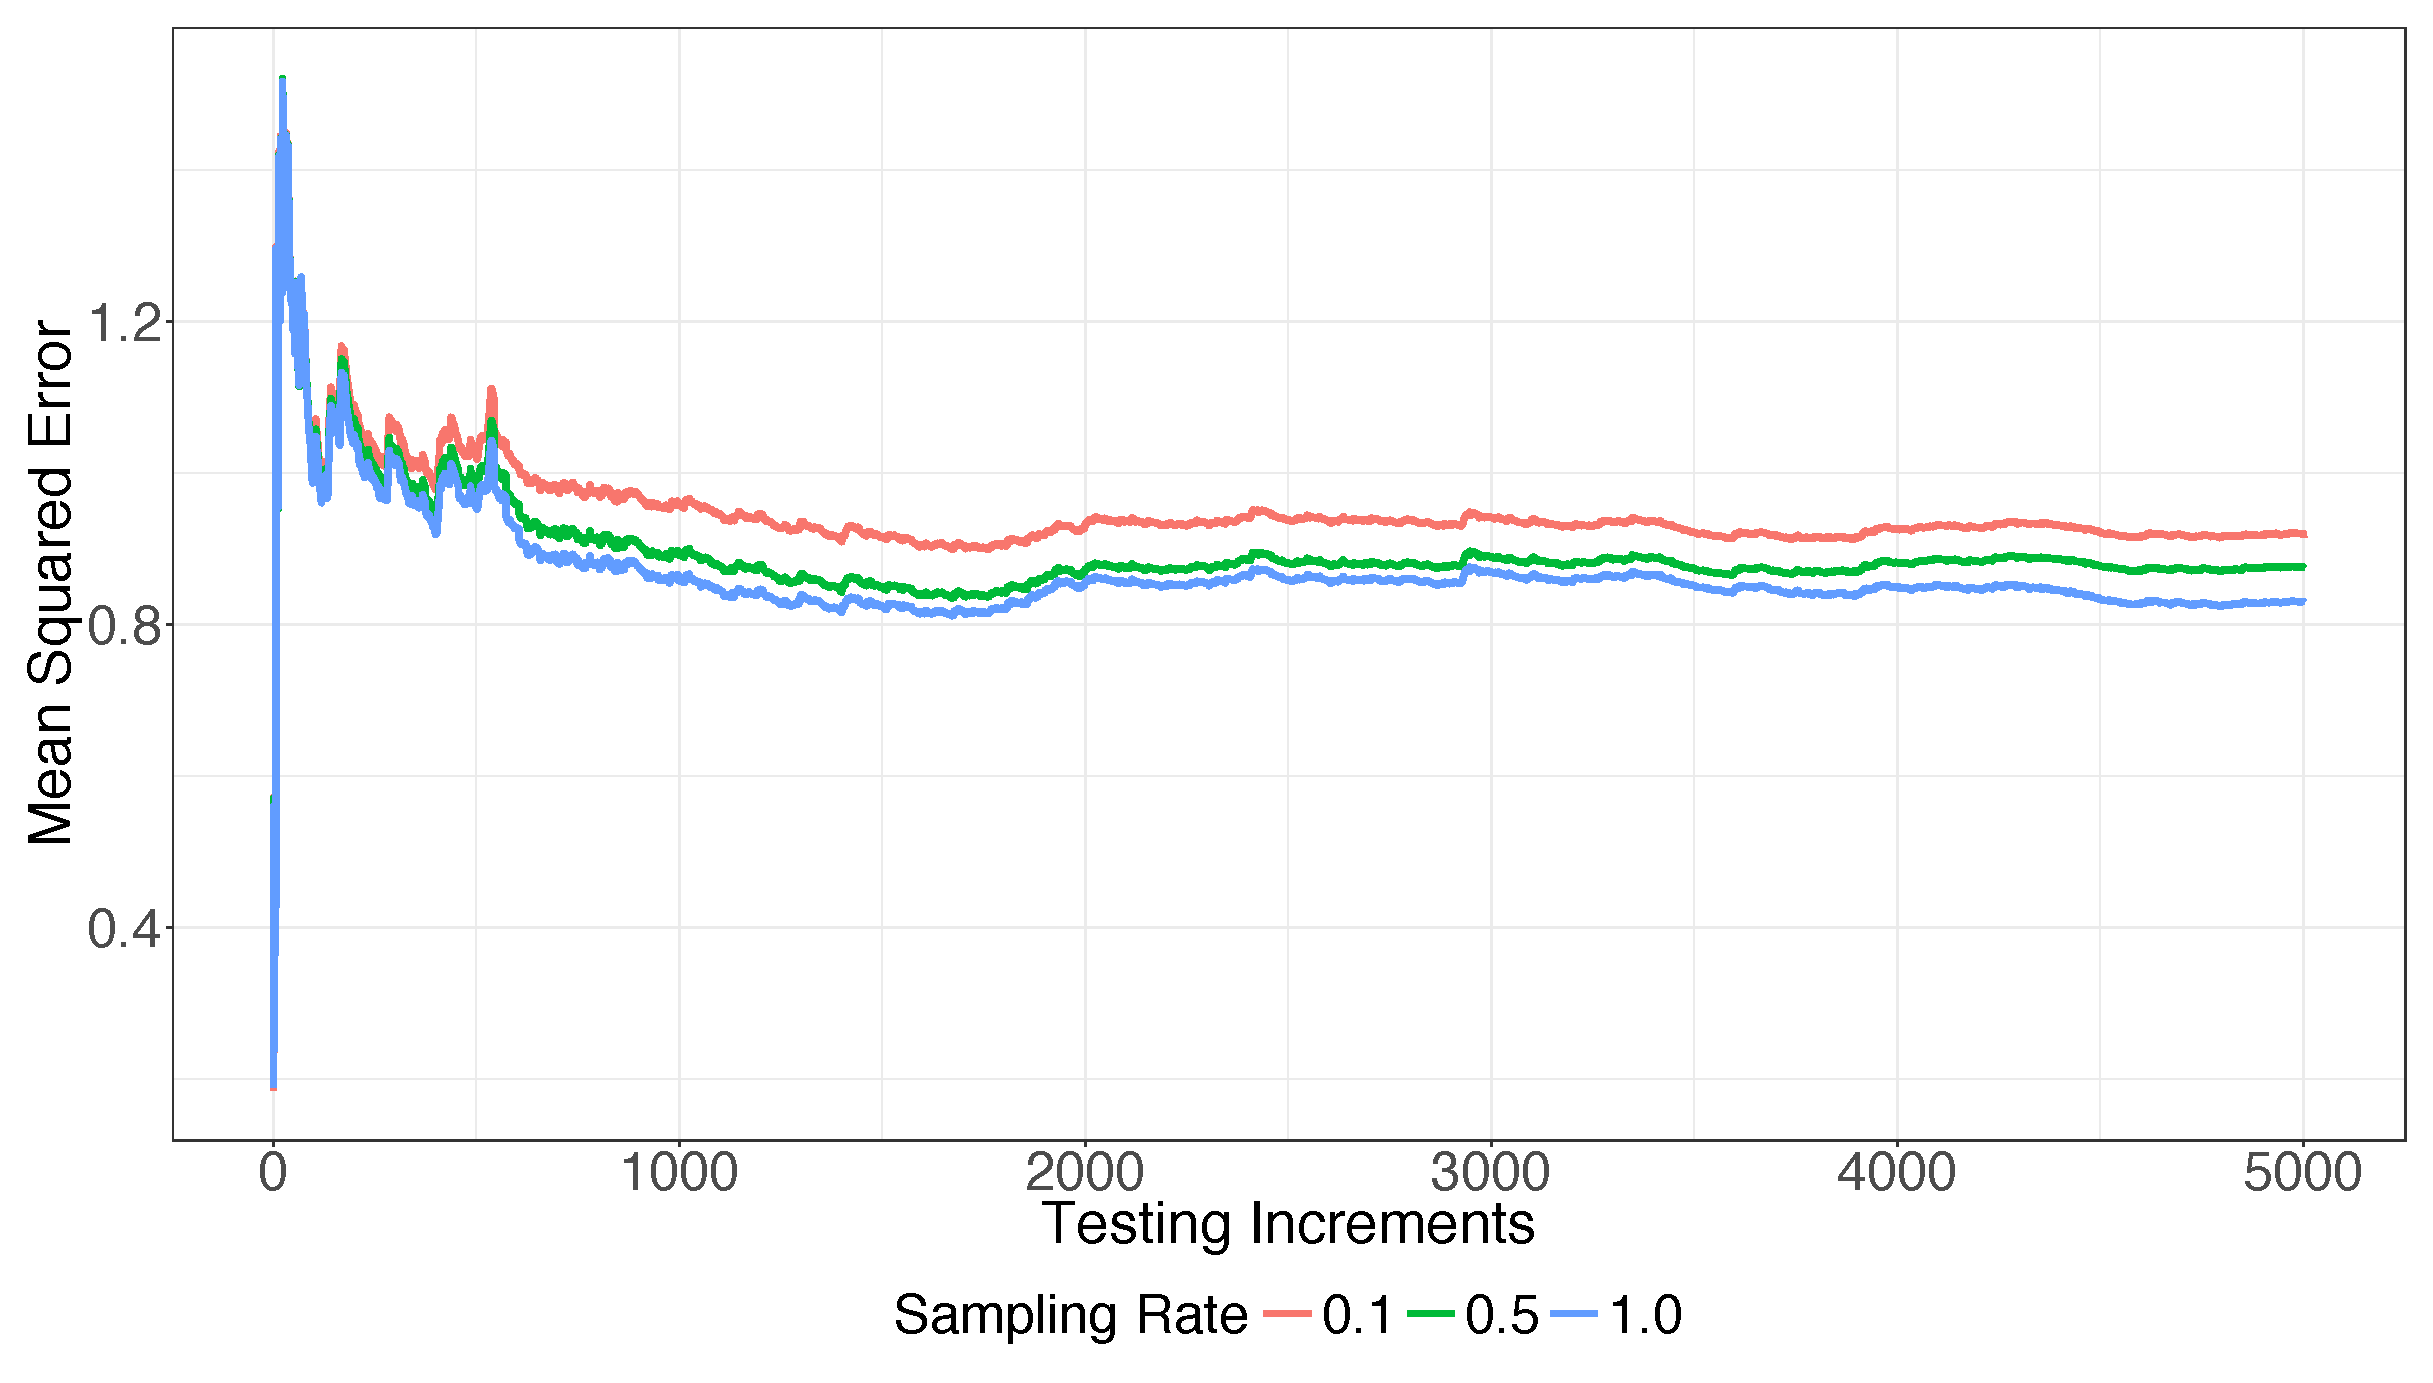
\includegraphics[width=\columnwidth]{../images/experiment-results/movie-lens-sampling-quality-improved.eps}
\caption{Sampling rate}
\label{fig:movie-lens-100k-sample-rate}
\end{subfigure}
\vspace{2mm}
\caption{Effect of Sampling and Scheduling Rate on Quality (Movie Lens 100K)}
\end{figure}

Figure \ref{fig:movie-lens-100k-buffer-size-mse} shows the mean squared error for different buffer sizes for Movie Lens 100k. 
A smaller buffer size forces the scheduler to initiate training iterations more frequently.
As a result, the system updates the underlying model more often.
However, the error rate is not decreasing linearly with the buffer size.
Further analysis shows that the more frequent the model updates are, the faster the model converges and any further training has little to no effect on the overall quality.
This is extremely important, specially when considering the effect of the buffer size on the running time.
Figure \ref{fig:movie-lens-100k-buffer-size-time} shows the running time on Movie Lens 100k using different buffer sizes. 
Increasing the buffer size from 500 to 5000 decreases the running time by a factor of 5 while the MSE is only decreased slightly.
Therefore, depending on the application, we can set the buffer size to bigger values in order to increase the performance of the system without affecting the quality of the final model substantially.

\begin{figure}[H]
\begin{subfigure}{0.5\columnwidth}
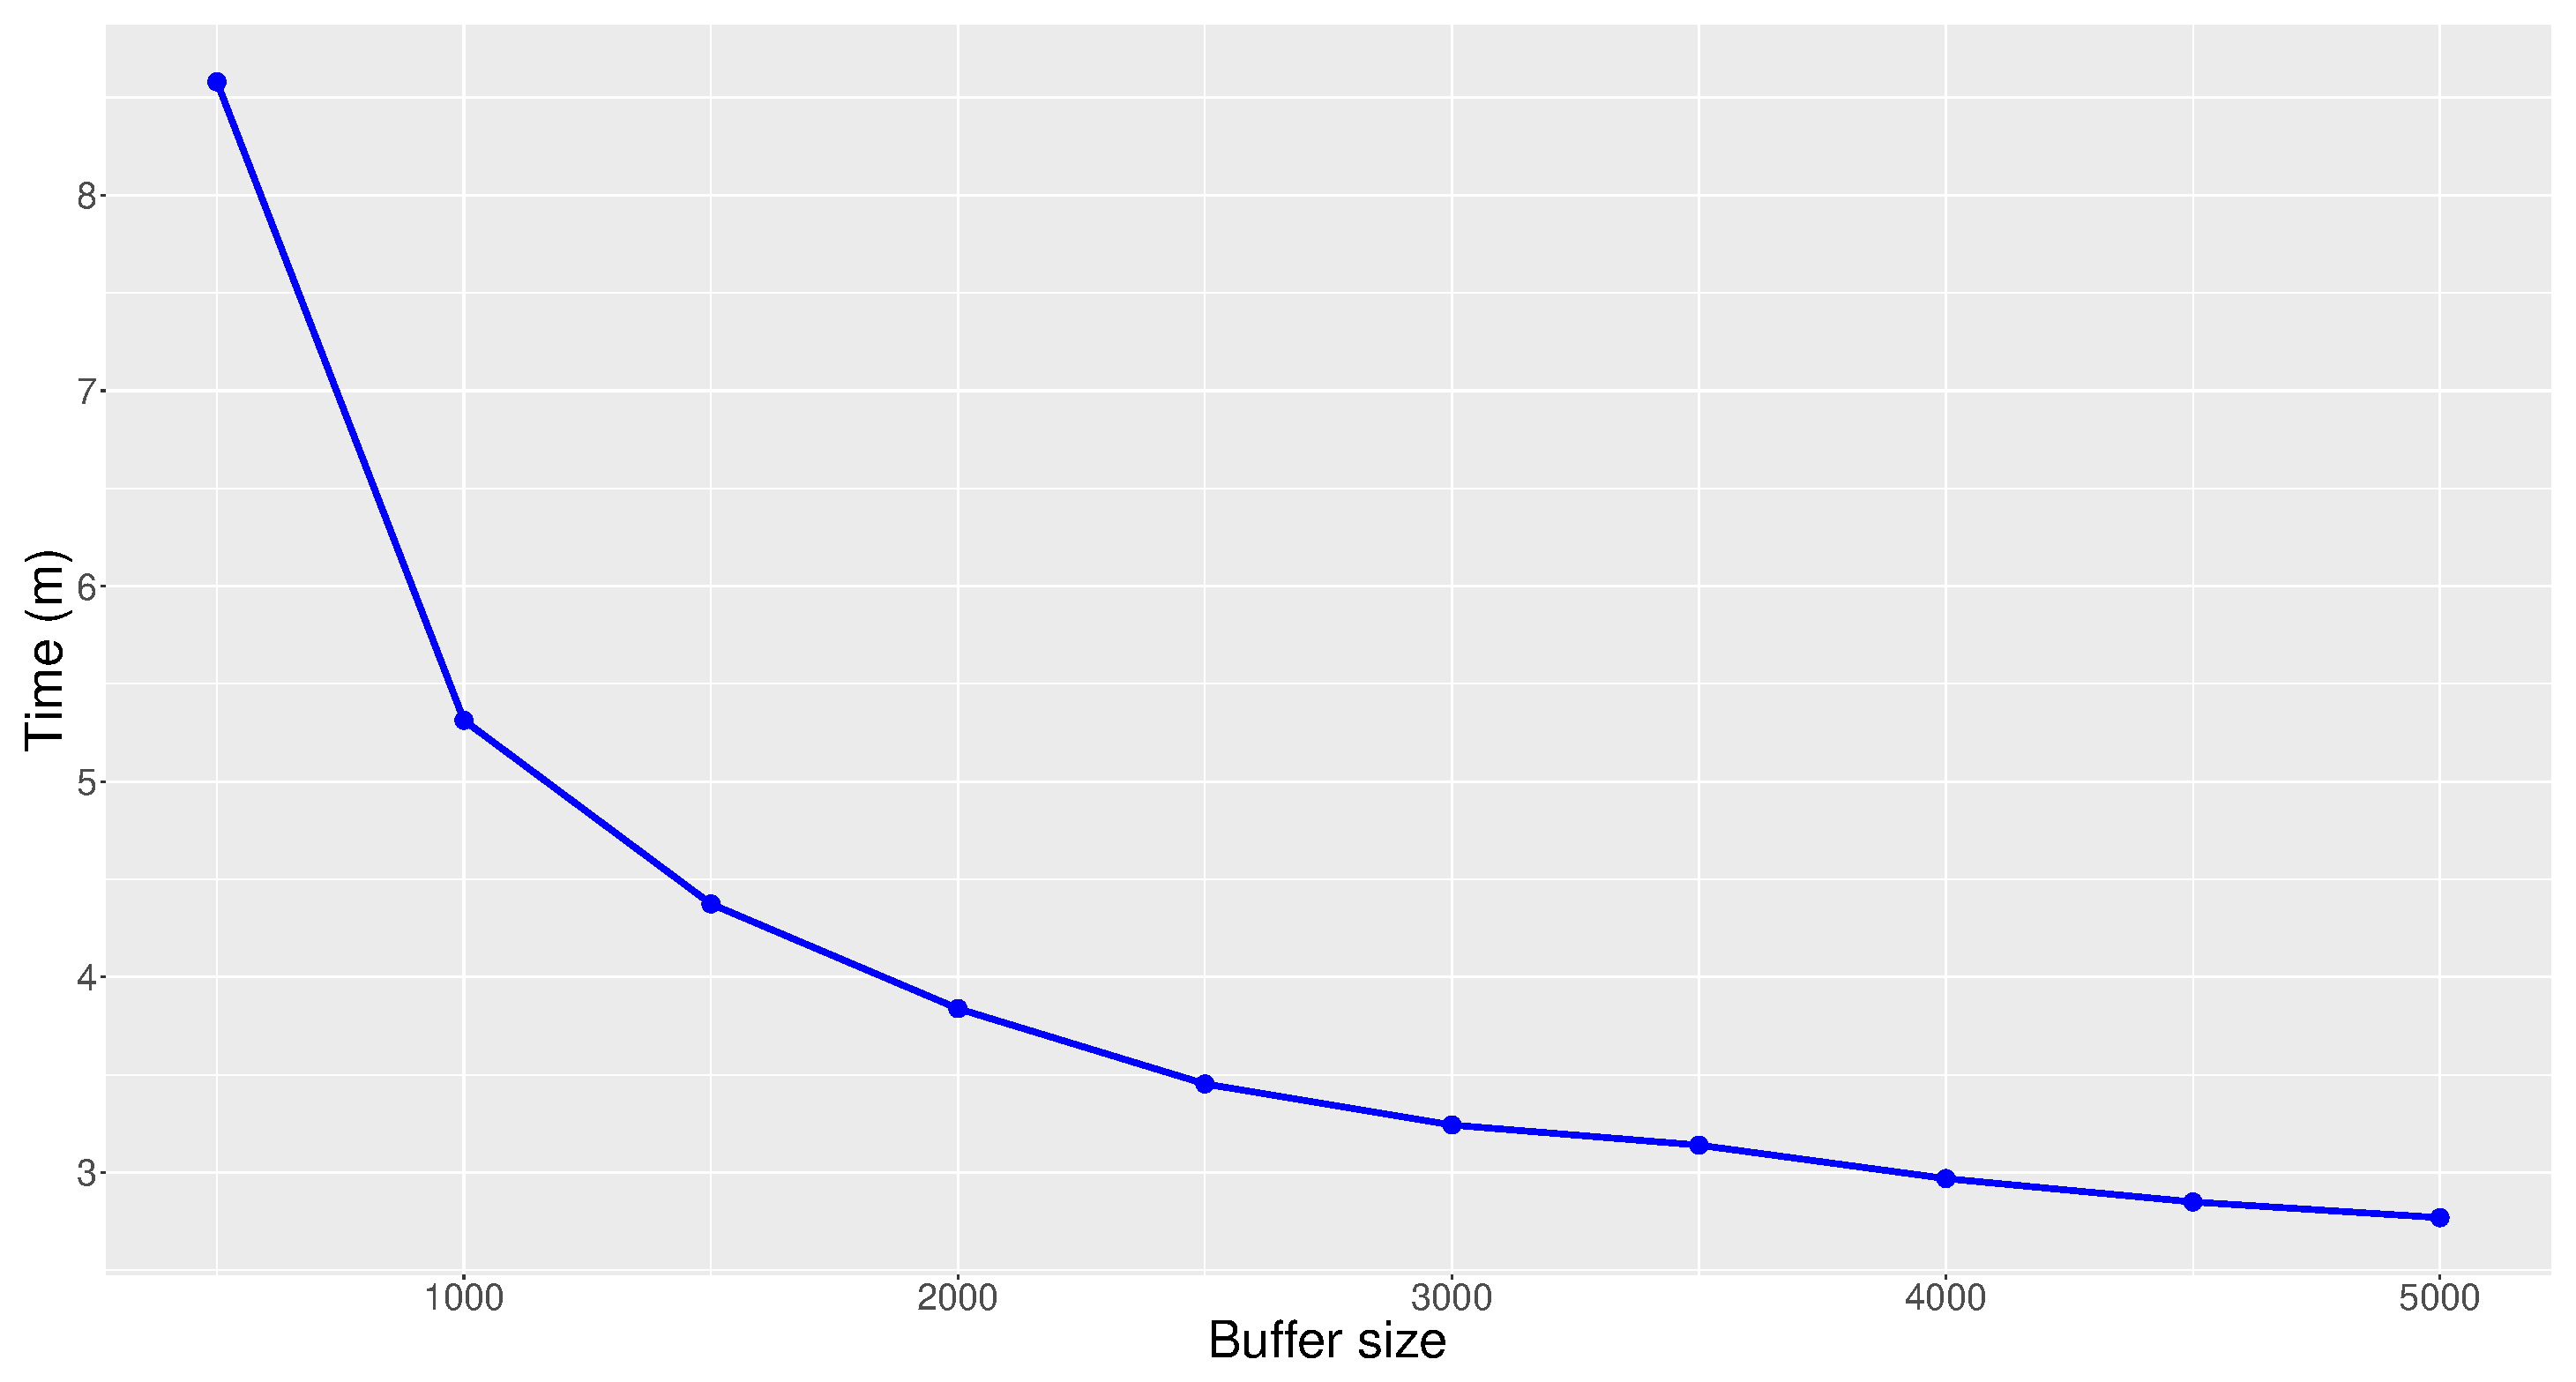
\includegraphics[width=\columnwidth]{../images/experiment-results/movie-lens-100k-buffer-time-improved.eps}
\caption{}
\label{fig:movie-lens-100k-buffer-size-time}
\end{subfigure}%
\begin{subfigure}{0.5\columnwidth}
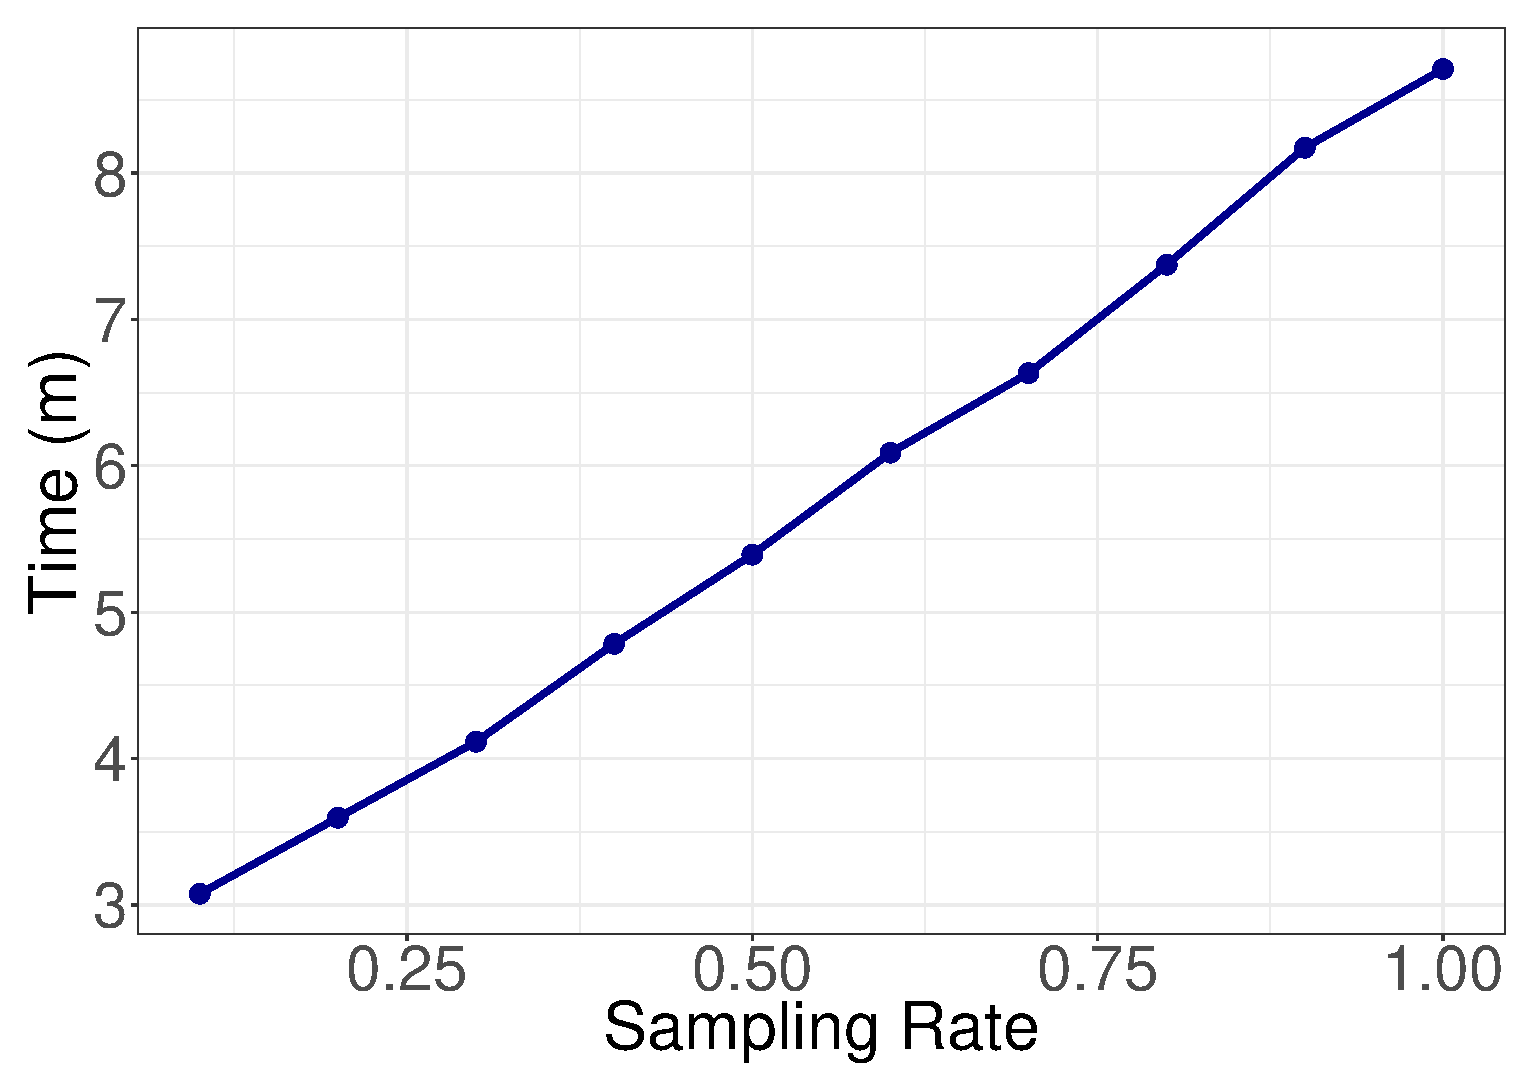
\includegraphics[width=\columnwidth]{../images/experiment-results/movie-lens-100k-sampling-time-improved.eps}
\caption{}
\label{fig:movie-lens-100k-sample-rate-time}
\end{subfigure}
\vspace{2mm}
\caption{Effect of Sampling and Scheduling Rate on Running time (Movie Lens 100K)}
\end{figure}

\todo[inline]{R1: Dynamic Scheduling is an interesting idea -- but you're not offering any scheduling algorithm here? Just the idea that you can schedule training when there's free CPU cycles? BD: Scheduling and Sampling rate have to be studied in more detail. All reviewers had concerns about these}
\todo[inline]{R3: What is exactly the scheduling?}
\textit{Dynamic scheduling:} In production environments, the load on the system typically varies throughout the lifetime of the application.
Therefore, a dynamic scheduling maximizes the performance of the system, by performing more frequent updates while there are more resources available for training. 
\todo[inline]{R1: "Moreover, since training and serving ... only update the weights when the training iteration is over". Why? Why not apply the updates to the model in-place? This allows you to serve every request with the absolute freshest model. At least for the single-machine case. BD: the updated model is the result of the training iterations, therefore, we have to wait until the iteration is over. The sentence seems clear to me. I should it run it by TR}
Moreover, since training and serving can be done in parallel, we can perform training in a background process and only update the weights when the training iteration is over. 


\subsection{Prediction Quality}
Quality achieved continuous compared with retraining method.
\begin{figure}[h]
\centering
\includegraphics[width=\columnwidth]{../images/placeholder.jpeg}
\caption{Log Loss Continuous vs Daily retraining Criteo }
\label{fig:continuous-vs-daily-criteo}
\vspace{2mm}
\end{figure}


\subsection{Serving Metrics}
\textbf{Model Freshness. }
How recent the pipeline was trained. 
The lower the value, the better quality the predictions are since they are made by a more recent model.
\begin{figure}[h]
\centering
\includegraphics[width=\columnwidth]{../images/placeholder.jpeg}
\caption{Model Freshness for deployment scenarios}
\label{fig:model-freshness-criteo}
\vspace{2mm}
\end{figure}
\textbf{Prediction Latency. }

\subsection{Training Time}
Total time spent training the pipeline for each scenario.
\begin{figure}[h]
\centering
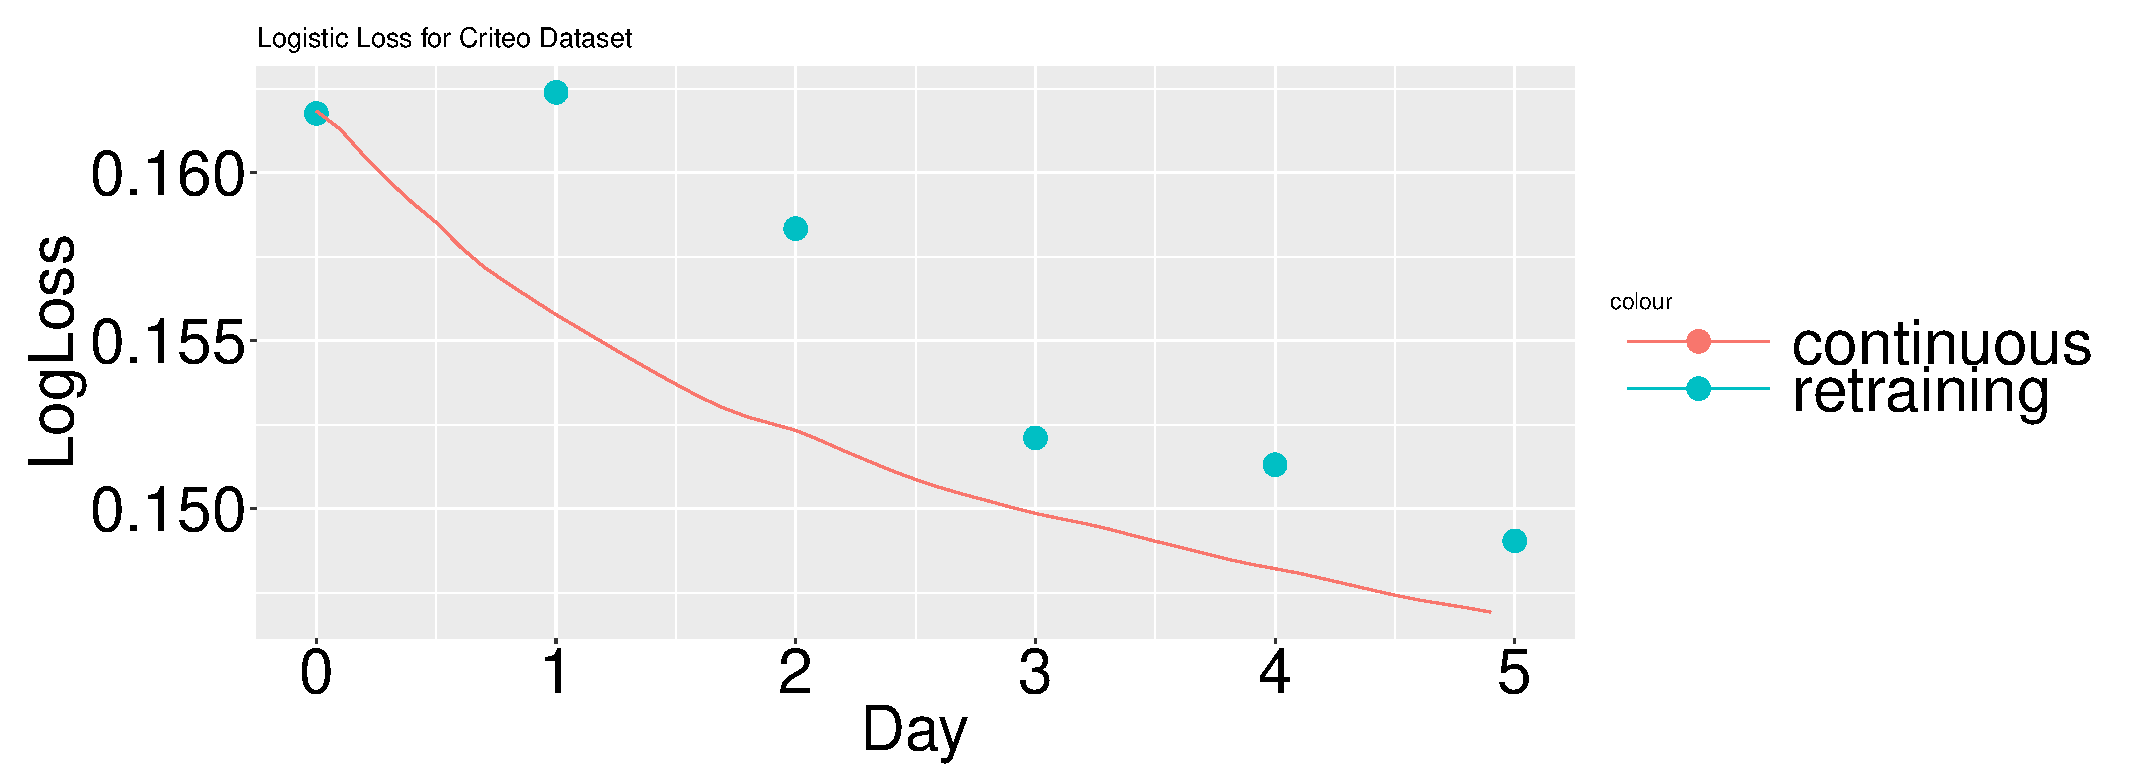
\includegraphics[width=\columnwidth]{../images/experiment-results/criteo-log-loss-continuous-vs-daily.eps}
\caption{Total training time of the pipeline for each scenario}
\label{fig:training-time-criteo}
\vspace{2mm}
\end{figure}

\subsection{Discussion} \label{subsec:discussion}
\begin{figure*}[t]
\begin{subfigure}{0.30\textwidth}
  \centering
  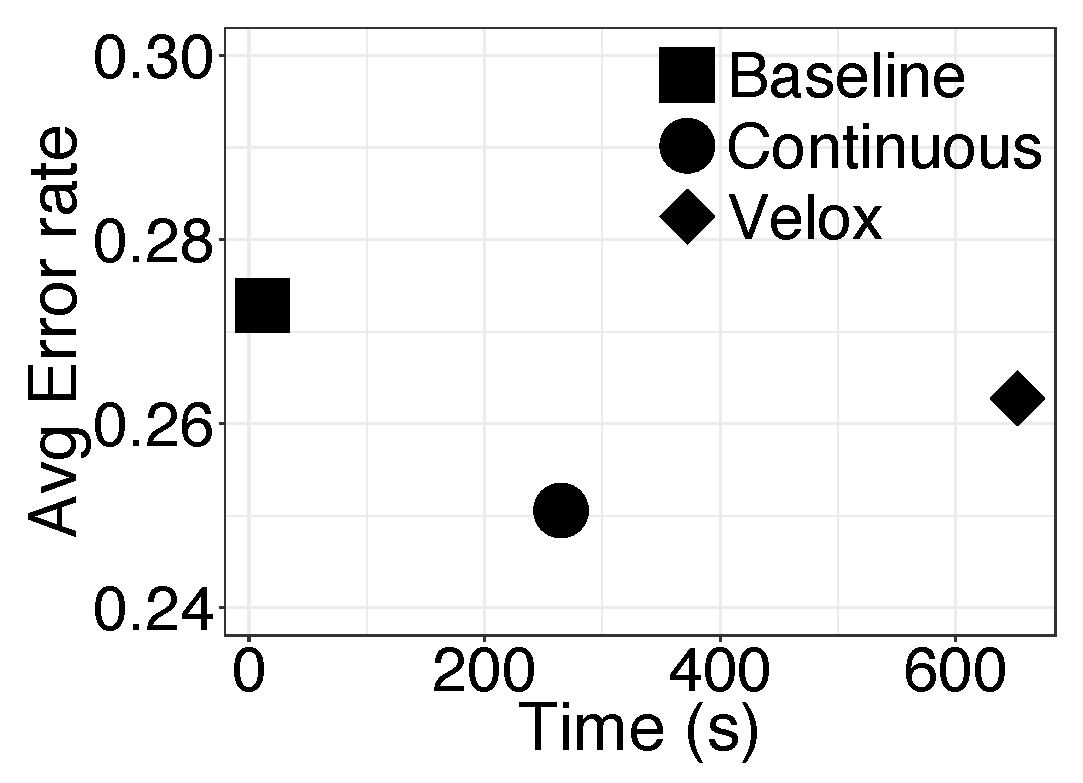
\includegraphics[width=\linewidth]{../images/experiment-results/cover-types-meta-performance.eps}
  \caption{Cover Type}
  \label{subfig:cover-type-meta}
\end{subfigure}%
  \hspace*{10mm}
\begin{subfigure}{0.30\textwidth}
 \centering
  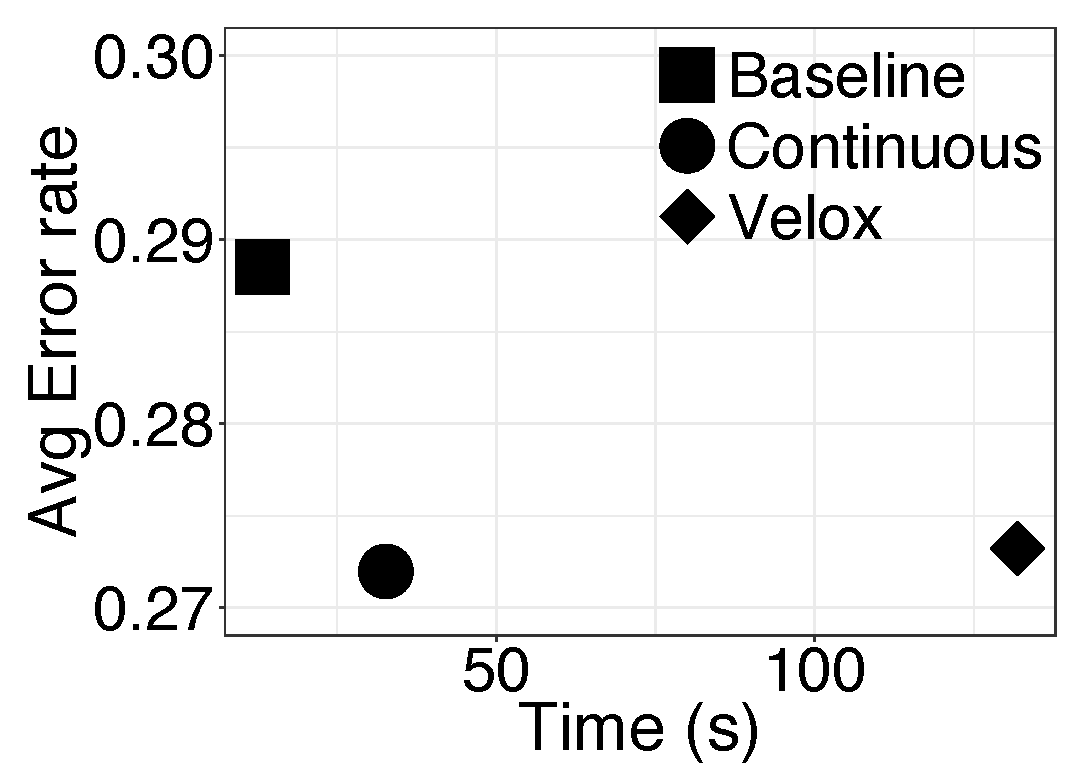
\includegraphics[width=\linewidth]{../images/experiment-results/sea-meta-performance.eps}
  \caption{SEA}
  \label{subfig:sea-meta}
\end{subfigure}%
 \hspace*{10mm}
 \begin{subfigure}{0.30\textwidth}
 \centering
  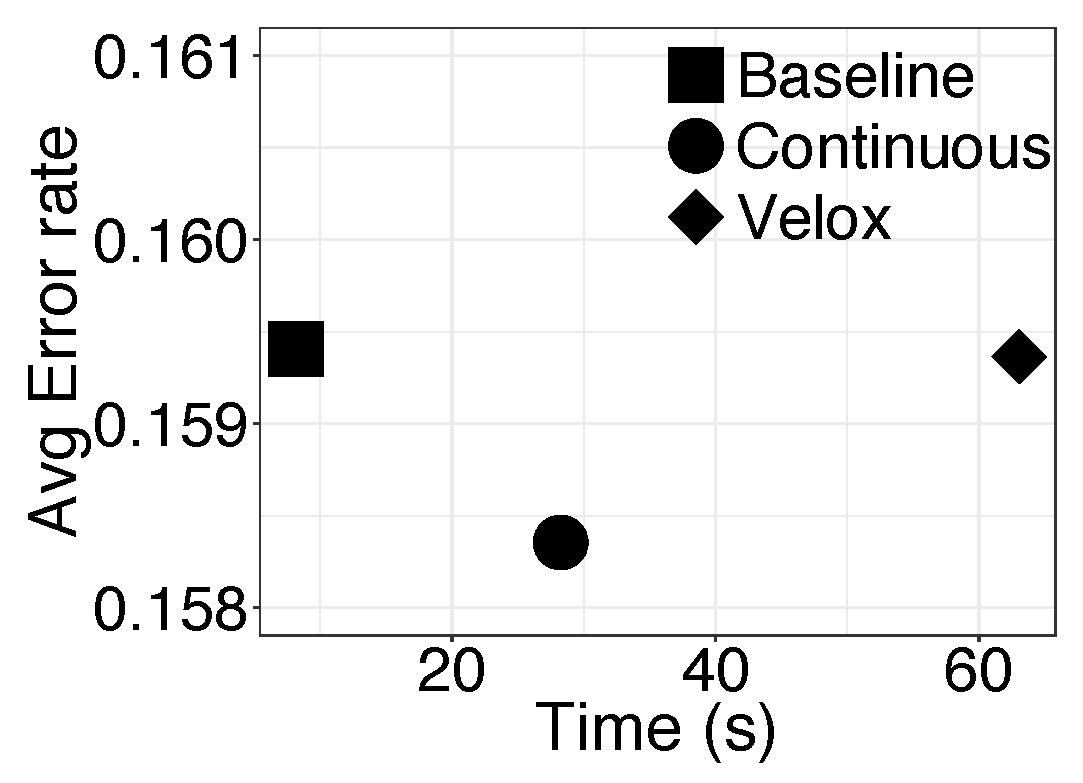
\includegraphics[width=\linewidth]{../images/experiment-results/adult-meta-performance.eps}
  \caption{Adult}
  \label{subfig:adult-meta}
\end{subfigure}%
 \vspace*{5mm}
\centering

\begin{subfigure}{.30\textwidth}
  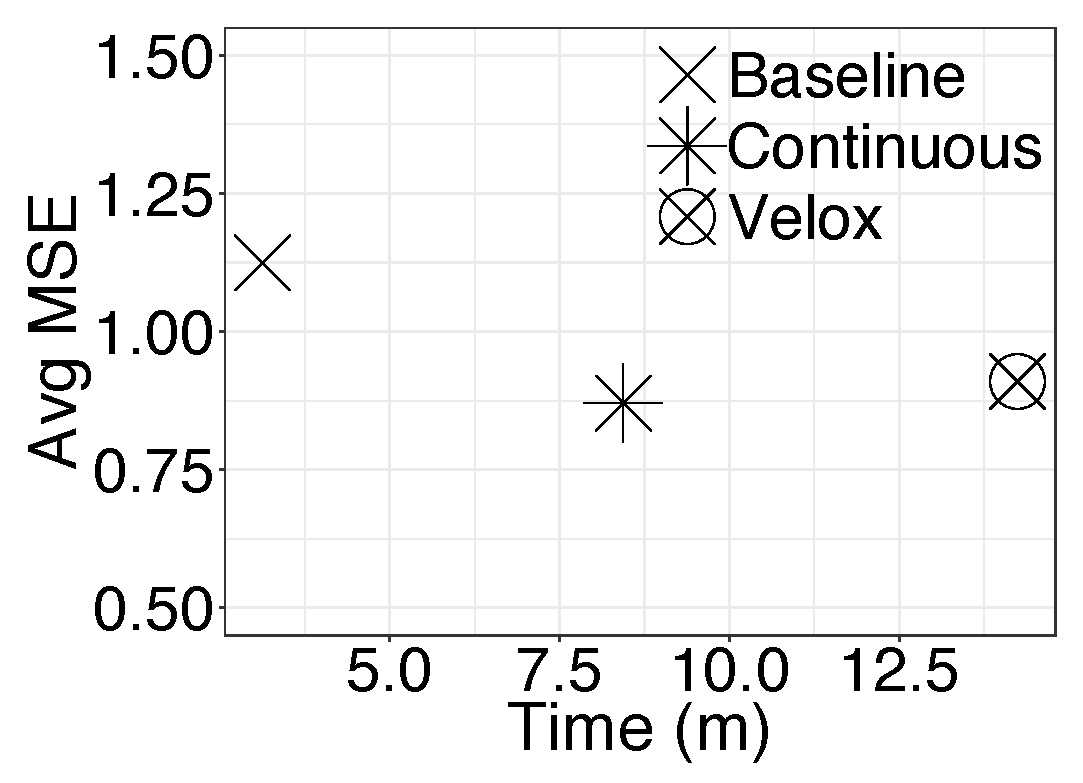
\includegraphics[width=1\linewidth, height=1\linewidth, keepaspectratio]{../images/experiment-results/movie-lens-100k-meta-performance.eps}
  \caption{Movie Lens 100K}
  \label{subfig:movie-lens-100k-meta}
\end{subfigure}%
 \hspace*{10mm}
\begin{subfigure}{0.30\textwidth}
  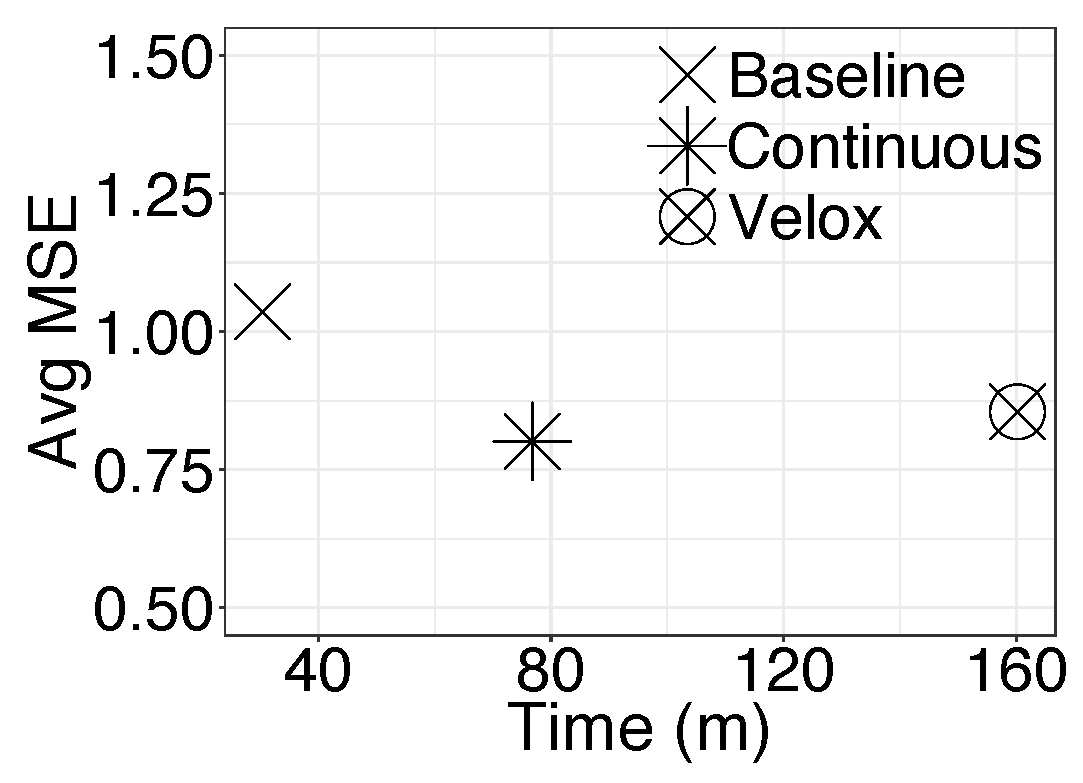
\includegraphics[width=1\linewidth, height=1\linewidth, keepaspectratio]{../images/experiment-results/movie-lens-1m-meta-performance.eps}
  \caption{Movie Lens 1M}
  \label{subfig:movie-lens-1m-meta}
\end{subfigure}


\begin{subfigure}{0.30\textwidth}
  \centering
  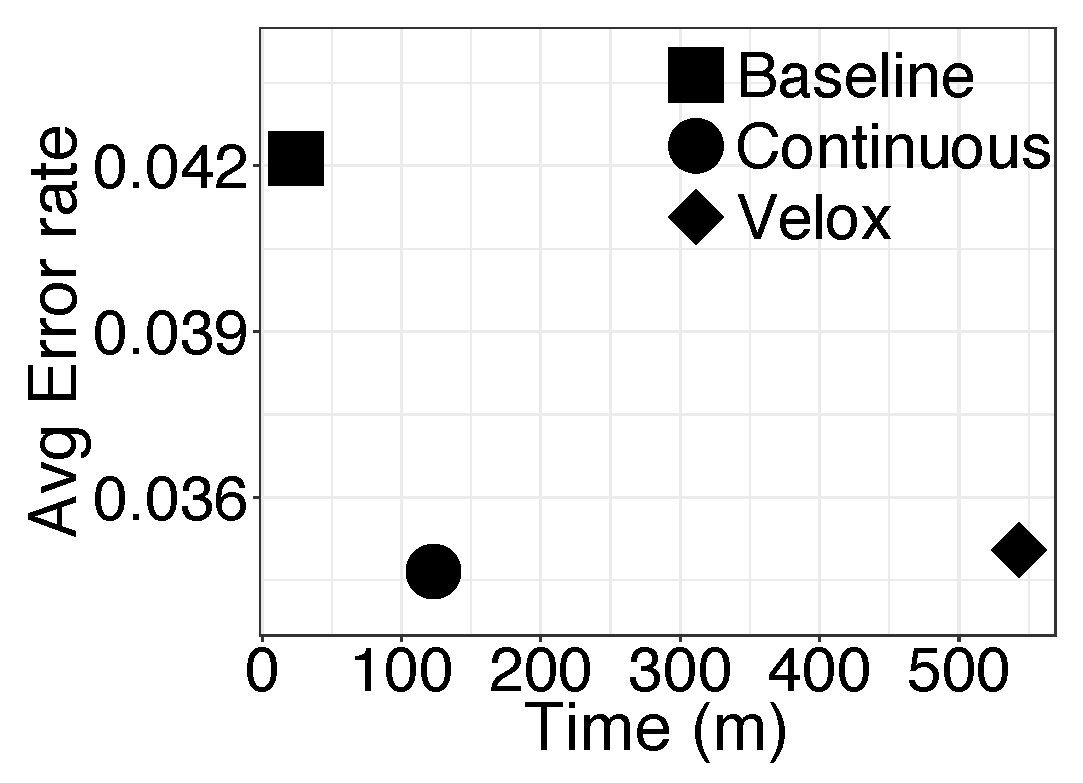
\includegraphics[width=\linewidth]{../images/experiment-results/url-reputation-meta-performance.eps}
  \caption{URL Reputation}
   \label{subfig:url-meta}
\end{subfigure}%
 \hspace*{10mm}
\begin{subfigure}{0.30\textwidth}
 \centering
  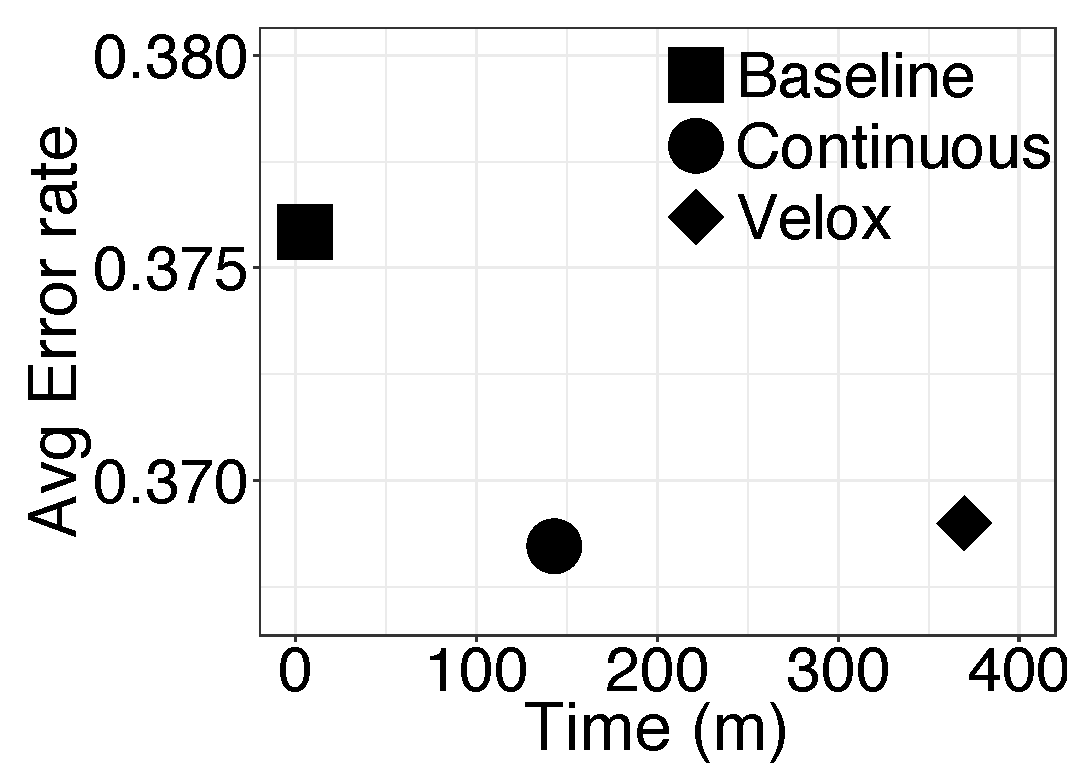
\includegraphics[width=\linewidth]{../images/experiment-results/higgs-meta-performance.eps}
  \caption{Higgs}
   \label{subfig:higgs-meta}
\end{subfigure}
 \vspace*{5mm}
\centering

\vspace{2mm}
\caption{Total Training Time vs Quality}
\label{fig:training-time-vs-quality}
\end{figure*}

Figure \ref{fig:training-time-vs-quality} shows the total training time and average error rate of each of the three different deployment methods (Baseline, Continuous, and Velox) on different datasets.
For all of the evaluated datasets, Continuous achieves the lowest average error rate (for the classification datasets) and average mean squared error (for the recommender system datasets).

The difference in average error rate (or average MSE) between Velox and Continuous is smaller for datasets that contain concept drift (Figure \ref{subfig:sea-meta}, \ref{subfig:movie-lens-100k-meta}, \ref{subfig:movie-lens-1m-meta}, and \ref{subfig:url-meta}).
Since both Velox and Continuous perform incremental and batch training of the model after it is deployed, they both manage to handle the concept drift in the data.
However, Continuous is able to adapt to the changes faster as it is continuously updating the model by executing iterations of SGD.
Since the retraining process is resource intensive, Velox cannot execute it frequently.
As a result, the underlying model in Velox cannot adapt to the changes in the distribution as quickly as Continuous.
The performance of Baseline is very poor in datasets with concept drift.
This is expected, as the underlying model in Baseline is only trained on an initial dataset.
Therefore, it is not capable of adapting to the changes in the data.

Continuous performs very well for datasets with no concept drifts (Figure \ref{subfig:cover-type-meta},  \ref{subfig:adult-meta}, and \ref{subfig:higgs-meta}) as well.
For the Cover Type and Higgs datasets, Baseline does not converge on the initial dataset, therefore it has a higher error rate than Velox and Continuous.
Velox performs better than Baseline on Higgs and Cover Type, however, retraining on these two datasets causes the underlying model to overfit to the existing data.
As a result, the performance of the model is decreased after each retraining.
This leads to an overall lower average error rate than that of Continuous.

As expected, Baseline has the lowest training time for all the datasets since it only trains the model only once on the initial datasets.
The total training time for Continuous is 2 to 5 time smaller than Velox for every datasets.
This has a big impact on prediction latency and accuracy.
In our current prototype, we do not address the problem of the trade off between prediction latency and accuracy.
In our prototype, both prediction and model updates are managed by the same node.
As a result, the prediction component is paused until the SGD iteration (or retraining in the case of Velox) is executed.
Therefore, the system always answers each prediction query using the latest version of the model, although with a much greater delay.
However, in an actual model deployment system, model training and prediction answering are typically executed on separate nodes (or threads).
Therefore, any prediction request arriving at the system is answered immediately, although not with the latest version of the model.
Since the retraining time for Velox is large, a considerable percentage of prediction requests are always answered by an older version of the model.
As a result, while the system is executing a retraining, the error rate will continue to rise until the retraining is finished.
For example in the URL Reputation dataset, the average time of each retraining is 68 minutes in Velox, whereas the average time of each iteration of SGD is 1.5 minutes.
This means that in worst case scenario, the model that is answering a prediction request in Velox is outdated by 1 hour.
Our continuous deployment method reduces this delay since it is updating the underlying model constantly using smaller batches of data.

